%%%%%%%%%%%%%%%%%%%%%%%%%%%%%%%%%%%%%%%%%%%%%%%%%%%%%%%%%%%%%%%%%%%%%
% Mitschrieb vom 03.12.2013                                         %
%%%%%%%%%%%%%%%%%%%%%%%%%%%%%%%%%%%%%%%%%%%%%%%%%%%%%%%%%%%%%%%%%%%%%
\chapter{Fundamentalgruppe und Überlagerungen}
\section{Homotopie von Wegen}
\begin{figure}[ht]
    \centering
    \subfloat[$\gamma_1$ und $\gamma_2$ sind homotop, da man sie 
             \enquote{zueinander verschieben} kann.]{
        \documentclass[varwidth=true, border=2pt]{standalone}

\usepackage{pgfplots}
\usepackage{tikz}

\begin{document}
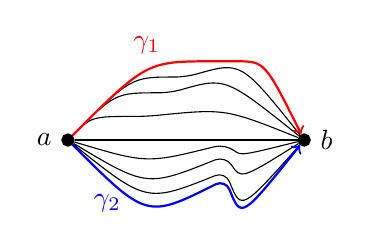
\begin{tikzpicture}
    \tikzstyle{point}=[circle,thick,draw=black,fill=black,inner sep=0pt,minimum width=4pt,minimum height=4pt]
    \node (a)[point,label=180:$a$] at (0,0) {};
    \node (b)[point,label=0:$b$]   at (3, 0) {};
    \draw [rounded corners] (a) .. controls (0.8,0.8) .. (1.5,0.8) .. controls (2.2,1) .. (b);
    \draw [rounded corners] (a) .. controls (0.6,0.6) .. (1.3,0.6) .. controls (2.0,0.8) .. (b);
    \draw [rounded corners] (a) .. controls (0.3,0.3) .. (1.0,0.3) .. controls (2.0,0.4) .. (b);
    \draw [rounded corners] (a) -- (b);
    \draw [rounded corners] (a) .. controls (1,-0.8) .. (2,-0.4) .. controls (2.2,-0.9) .. (b);
    \draw [rounded corners] (a) .. controls (1,-0.6) .. (2,-0.2) .. controls (2.2,-0.5) .. (b);
    \draw [rounded corners] (a) .. controls (1,-0.3) .. (2,-0.05) .. controls (2.2,-0.2) .. (b);
    \draw [rounded corners,->, thick, red] (a) .. controls (1,1) .. (2,1) .. controls (2.5,1) .. (b);
    \draw [rounded corners,->, thick, blue] (a) .. controls (1,-1) .. (2,-0.5) .. controls (2.2,-1) .. (b);
    \node at (1,1.2) [red] {$\gamma_1$};
    \node at (0.5,-0.8) [blue] {$\gamma_2$};
\end{tikzpicture}
\end{document}

        \label{fig:homotope-wege-anschaulich}
    }\hspace{1em}%
    \subfloat[$\gamma_1$ und $\gamma_2$ sind wegen dem Hindernis nicht homotop.]{
        \begin{tikzpicture}
    \tikzstyle{point}=[circle,thick,draw=black,fill=black,inner sep=0pt,minimum width=4pt,minimum height=4pt]
    \node (a)[point,label=180:$a$] at (0,0) {};
    \node (b)[point,label=0:$b$]   at (3, 0) {};
    \draw[orange,pattern color=orange,pattern=north east lines] (1.5,0) circle (0.3cm);
    \draw [rounded corners,->, thick, red] (a) .. controls (1,1) .. (2,1) .. controls (2.5,1) .. (b);
    \draw [rounded corners,->, thick, blue] (a) .. controls (1,-1) .. (2,-0.5) .. controls (2.2,-1) .. (b);
    \node at (1,1.2) [red] {$\gamma_1$};
    \node at (0.5,-0.8) [blue] {$\gamma_2$};
\end{tikzpicture}

        \label{fig:nicht-homotope-wege-anschaulich}
    }
    \label{fig:paths-homotop-example-counterexample}
    \caption{Beispiele für Wege $\gamma_1$ und $\gamma_2$}
\end{figure}

\begin{definition}
    Sei $X$ ein topologischer Raum, $a, b \in X$, 
    $\gamma_1, \gamma_2: [0,1] \rightarrow X$ Wege von $a$ nach $b$,
    d.~h. $\gamma_1(0) = \gamma_2(0) = a$, $\gamma_1(1) = \gamma_2(1) = b$

    \begin{defenum}
        \item $\gamma_1$ und $\gamma_2$ heißen \textbf{homotop}\xindex{Weg!homotope},
              wenn es eine stetige Abbildung $H : I \times I \rightarrow X$ mit
              \[H(t,0) = \gamma_1(t), H(t,1) = \gamma_2(t) \;\;\; \forall t \in [0,1] =: I \]
              und $H(0,s) = a$ und $H(1,s) = b$ für alle $s \in I$ gibt.
              Dann schreibt man: $\gamma_1 \sim \gamma_2$

              $H$ heißt \textbf{Homotopie}\xindex{Homotopie} zwischen
              $\gamma_1$ und $\gamma_2$.
        \item $\gamma_s: I \rightarrow X, \gamma_s(t) = H(t,s)$ ist
              Weg in $X$ von $a$ nach $b$ für jedes $s \in I$.
    \end{defenum}
\end{definition}

\begin{bemerkung}
    \enquote{Homotop} ist eine Äquivalenzrelation auf der Menge aller
    Wege in $X$ von $a$ nach $b$.
\end{bemerkung}

\begin{beweis}\leavevmode
    \begin{itemize}
        \item reflexiv: $H(t,s) = \gamma(t)$ für alle $(t,s) \in I \times I$
        \item symmetrisch: $H'(t,s) = H(t,1-s)$ für alle $(t,s) \in I \times I$
        \item transitiv: Seien $H'$ bzw. $H''$ Homotopien von $\gamma_1$
              nach $\gamma_2$ bzw. von $\gamma_2$ nach $\gamma_3$.

              Dann sei $H(t,s) := \begin{cases}
              H'(t, 2s)    &\text{falls } 0 \leq s \leq \frac{1}{2}\\
              H''(t, 2s-1) &\text{falls } \frac{1}{2} \leq s \leq 1\end{cases}$

              $\Rightarrow$ $H$ ist stetig und Homotopie von $\gamma_1$ nach 
              $\gamma_3$.
    \end{itemize}
    $\qed$
\end{beweis}

\begin{beispiel}
    \begin{bspenum}
        \item Sei $X = S^1$. $\gamma_1$ und $\gamma_2$ aus 
              \cref{fig:circle-two-paths} nicht homotop.
        \item Sei $X = T^2$. $\gamma_1, \gamma_2$ und $\gamma_3$
              aus \cref{fig:torus-three-paths} sind paarweise
              nicht homotop.
        \item Sei $X = \mdr^2$ und $a=b=(0,0)$. 

              Je zwei Wege im $\mdr^2$ mit Anfangs- und Endpunkt $(0,0)$
              sind homotop.

              \begin{figure}[htp]
                \centering
                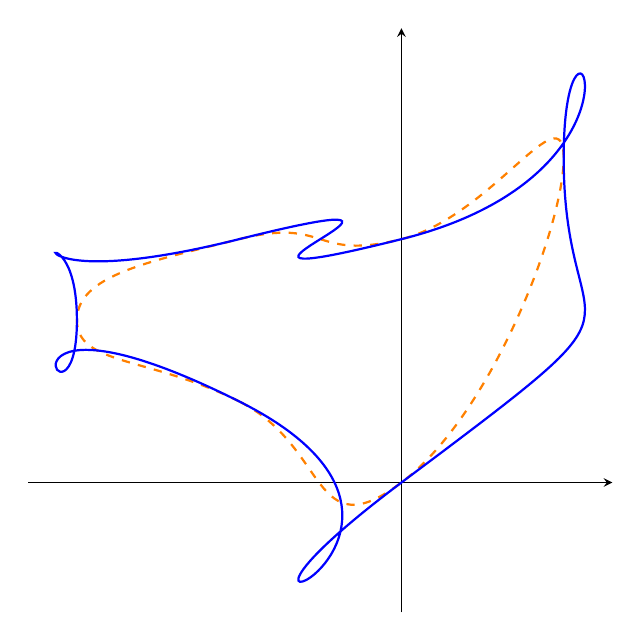
\begin{tikzpicture}
    \begin{axis}[
        legend pos=south west,
        axis x line=middle,
        axis y line=middle,
        %grid = major,
        width=9cm,
        height=9cm,
        grid style={dashed, gray!30},
        xmin=-2,     % start the diagram at this x-coordinate
        xmax= 1,    % end   the diagram at this x-coordinate
        ymin=-1,     % start the diagram at this y-coordinate
        ymax= 5,   % end   the diagram at this y-coordinate
        %axis background/.style={fill=white},
        %xlabel=$x$,
        %ylabel=$y$,
        ticks=none,
        %tick align=outside,
        %minor tick num=-3,
        enlargelimits=true,
        tension=0.08]
        \addplot[mark=none, orange, smooth cycle, thick, tension=1, dashed] coordinates {%
   (0,0) (-1,1) (-2,2) (-1,3) (0, 3) (1, 4)};
        \addplot[mark=none, blue, smooth cycle, thick, tension=3] coordinates {%
   (0,0) (-1,1) (-2,2) (-1,3) (0, 3) (1, 4)};
    \end{axis} 
\end{tikzpicture}

                \caption{Zwei Wege im $\mdr^2$ mit Anfangs- und Endpunkt $(0,0)$}
                \label{fig:paths-from-origin}
              \end{figure}

              Sei $\gamma_0: I \rightarrow \mdr^2$ der konstante Weg
              $\gamma_0(t) = (0,0) \; \forall t \in I$. Sei
              $\gamma(0) = \gamma(1) = (0,0)$.

              $H(t,s) := (1-s) \gamma(t)$ ist stetig, 
              $H(t,0) = \gamma(t)\; \forall t \in I$ und
              $H(t,1) = (0,0) \; \forall t \in I$.
    \end{bspenum}

    \begin{figure}[ht]
        \centering
        \subfloat[Kreis mit zwei Wegen]{
            \documentclass[varwidth=true, border=2pt]{standalone}

\usepackage{pgfplots}
\usepackage{tikz}

\begin{document}
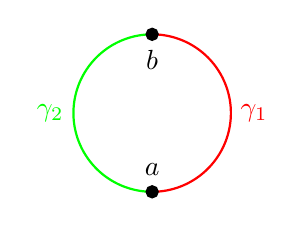
\begin{tikzpicture}
    \tikzstyle{point}=[circle,thick,draw=black,fill=black,inner sep=0pt,minimum width=4pt,minimum height=4pt]
    \draw [red,  thick,domain=90:-90,  samples=100] plot ({cos(\x)}, {sin(\x)});
    \draw [green,thick,domain=-90:-270,samples=100] plot ({cos(\x)}, {sin(\x)});
    \node (a)[point,label=90:$a$] at (0,-1cm) {};
    \node (b)[point,label=-90:$b$] at (0, 1cm) {};

    \node at (1,0) [anchor=180, red] {$\gamma_1$};
    \node at (-1,0) [anchor=0, green] {$\gamma_2$};

\end{tikzpicture}
\end{document}

            \label{fig:circle-two-paths}
        }%
        \subfloat[Torus mit drei Wegen]{
            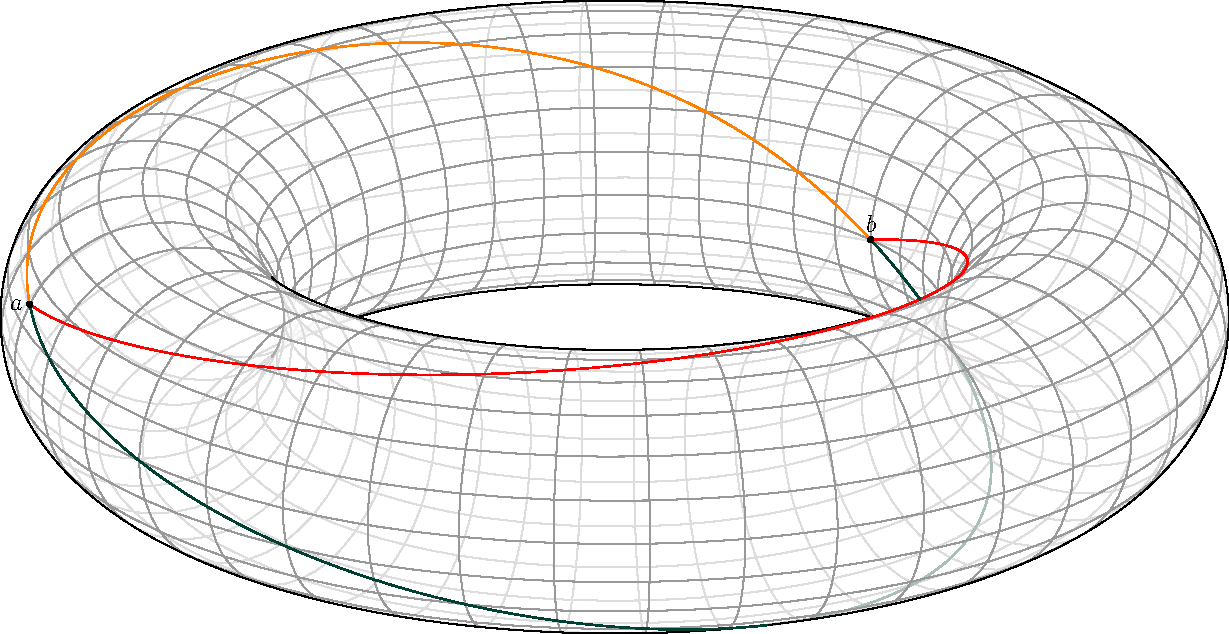
\includegraphics[width=0.45\linewidth, keepaspectratio]{figures/torus-three-paths.pdf}
            \label{fig:torus-three-paths}
        }%
        \label{fig:homotop-paths}
        \caption{Beispiele für (nicht)-Homotopie von Wegen}
    \end{figure}
\end{beispiel}

%%%%%%%%%%%%%%%%%%%%%%%%%%%%%%%%%%%%%%%%%%%%%%%%%%%%%%%%%%%%%%%%%%%%%
% Mitschrieb vom 05.12.2013                                         %
%%%%%%%%%%%%%%%%%%%%%%%%%%%%%%%%%%%%%%%%%%%%%%%%%%%%%%%%%%%%%%%%%%%%%
\begin{bemerkung}\label{kor:homotope-wege}
    Sei $X$ ein topologischer Raum, $\gamma: I \rightarrow X$ ein 
    Weg und $\varphi: I \rightarrow I$ stetig mit $\varphi(0) = 0$,
    $\varphi(1) = 1$. Dann sind $\gamma$ und $\gamma \circ \varphi$
    homotop.
\end{bemerkung}

\begin{beweis}
    Sei $H (t,s) = \gamma ((1-s) t + s \cdot \varphi(t))$.

    Dann ist $H$ stetig, $H(t,0) = \gamma(t),\;\;\; H(t,1) = \gamma ( \varphi(t)),\;\;\;$
    $H(0,s) = \gamma(0)$ und $H(1,s) = \gamma(1-s+s) = \gamma(1)$\\
    $\Rightarrow H$ ist Homotopie. $\qed$
\end{beweis}

\begin{definition}\xindex{Weg!zusammengesetzter}
    Seien $\gamma_1, \gamma_2$ Wege in $X$ mit $\gamma_1(1) = \gamma_2(0)$.
    Dann ist 
    \[\gamma (t) = \begin{cases}
        \gamma_1(2t)   &\text{falls} 0 \leq t < \frac{1}{2}\\
        \gamma_2(2t-1) &\text{falls} \frac{1}{2} \leq t \leq 1
      \end{cases}\]
    ein Weg in $X$. Er heißt \textbf{zusammengesetzter Weg} und man
    schreibt $\gamma = \gamma_1 * \gamma_2$.
\end{definition}

\begin{bemerkung}\label{kor:assoziativitaet-von-zusammensetzen-von-wegen}
    Das Zusammensetzen von Wegen ist nur bis auf 
    Homotopie assoziativ, d.~h.:
    \begin{align*}
        \gamma_1 * (\gamma_2 * \gamma_3) &\neq (\gamma_1 * \gamma_2) * \gamma_3\\
        \gamma_1 * (\gamma_2 * \gamma_3) &\sim (\gamma_1 * \gamma_2) * \gamma_3
    \end{align*}
    mit $\gamma_1(1)=\gamma_2(0)$ und $\gamma_2(1) = \gamma_3(0)$.
\end{bemerkung}

\begin{beweis}
    \begin{figure}[ht]
        \centering
        \subfloat[$\gamma_1 * (\gamma_2 * \gamma_3)$]{
            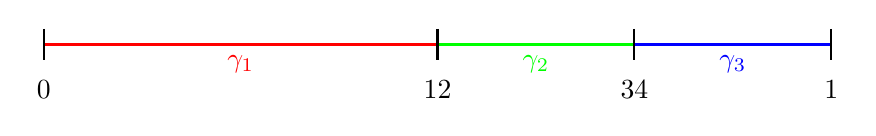
\begin{tikzpicture}
    \draw[very thick,red]   (0,0) -- (5,0) node [midway, below] {$\gamma_1$};
    \draw[very thick,green](5,0) -- (7.5,0) node [midway, below] {$\gamma_2$};
    \draw[very thick,blue] (7.5,0) -- (10,0) node [midway, below] {$\gamma_3$};

    \draw[thick] (0,0.2)   -- (  0,-0.2) node[label=below:$0$] {};
    \draw[thick] (5,0.2)   -- (  5,-0.2) node[label=below:$\nicefrac{1}{2}$] {};
    \draw[thick] (7.5,0.2) -- (7.5,-0.2) node[label=below:$\nicefrac{3}{4}$] {};
    \draw[thick] (10,0.2)  -- ( 10,-0.2) node[label=below:$1$] {};
\end{tikzpicture}

            \label{fig:assotiativitaet-von-wegen-a}
        }

        \subfloat[$(\gamma_1 * \gamma_2) * \gamma_3$]{
            \documentclass[varwidth=true, border=2pt]{standalone}
\usepackage{tikz}
\usepackage{nicefrac}

\begin{document}
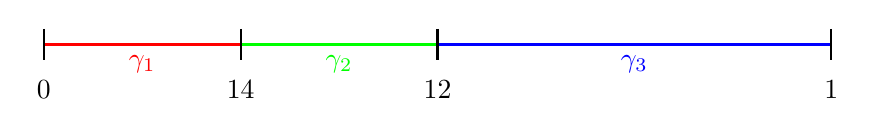
\begin{tikzpicture}
    \draw[very thick,red]   (0,0) -- (2.5,0) node [midway, below] {$\gamma_1$};
    \draw[very thick,green](2.5,0) -- (5,0) node [midway, below] {$\gamma_2$};
    \draw[very thick,blue] (5,0) -- (10,0) node [midway, below] {$\gamma_3$};

    \draw[thick] (0,0.2)   -- (  0,-0.2) node[label=below:$0$] {};
    \draw[thick] (2.5,0.2) -- (2.5,-0.2) node[label=below:$\nicefrac{1}{4}$] {};
    \draw[thick] (5.0,0.2) -- (5.0,-0.2) node[label=below:$\nicefrac{1}{2}$] {};
    \draw[thick] (10,0.2)  -- ( 10,-0.2) node[label=below:$1$] {};
\end{tikzpicture}
\end{document}

            \label{fig:assotiativitaet-von-wegen-b}
        }%
        \label{fig:assoziativitaet-von-wegen}
        \caption{Das Zusammensetzen von Wegen ist nicht assoziativ}
    \end{figure}

    Das Zusammensetzen von Wegen ist wegen \cref{kor:homotope-wege}
    bis auf Homotopie assoziativ. Verwende dazu

    \[\varphi(t) = \begin{cases}
            \frac{1}{2} t   &\text{falls } 0 \leq t < \frac{1}{2}\\
            t - \frac{1}{4} &\text{falls } \frac{1}{2} \leq t < \frac{3}{4}\\
            2t - 1          &\text{falls } \frac{3}{4} \leq t \leq 1
        \end{cases}\]
\end{beweis}

\begin{bemerkung}\label{kor:bemerkung-10-6}
    Sei $X$ ein topologischer Raum, $a,b,c \in X$, $\gamma_1, \gamma_1'$
    Wege von $a$ nach $b$ und $\gamma_2, \gamma_2'$ Wege von $b$ nach $c$.

    Sind $\gamma_1 \sim \gamma_1'$ und $\gamma_2 \sim \gamma_2'$, so
    ist $\gamma_1 * \gamma_2 \sim \gamma_1 ' * \gamma_2'$.
\end{bemerkung}

\begin{figure}[htp]
    \centering
    \documentclass[varwidth=true, border=2pt]{standalone}

\usepackage{pgfplots}
\usepackage{tikz}

\begin{document}
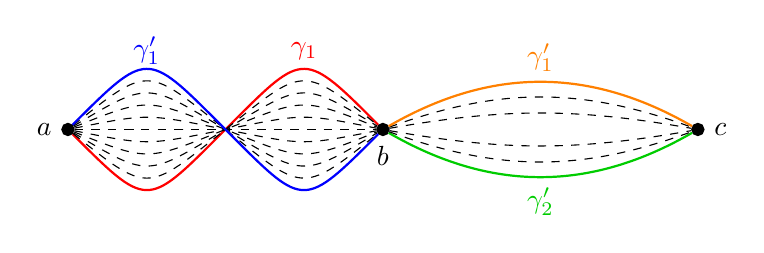
\begin{tikzpicture}
    \tikzstyle{point}=[circle,thick,draw=black,fill=black,inner sep=0pt,minimum width=4pt,minimum height=4pt]
    \node at (3,1) [red] {$\gamma_1$};
    \node at (1,1) [blue] {$\gamma_1'$};
    \node (a)[point,label=180:$a$] at (0,0) {};
    \node (b)[point,label=-90:$b$]   at (4, 0) {};
    \node (c)[point,label=0:$c$]   at (8, 0) {};
    \draw [rounded corners, thick, red] (a) .. controls (1,-1) .. (2,0)  .. controls (3,1) .. (b);
    \draw [rounded corners, dashed] (a) .. controls (1,-0.8) .. (2,0) .. controls (3,0.8) .. (b);
    \draw [rounded corners, dashed] (a) .. controls (1,-0.6) .. (2,0) .. controls (3,0.6) .. (b);
    \draw [rounded corners, dashed] (a) .. controls (1,-0.4) .. (2,0) .. controls (3,0.4) .. (b);
    \draw [rounded corners, dashed] (a) .. controls (1,-0.2) .. (2,0) .. controls (3,0.2) .. (b);
    \draw [rounded corners, dashed] (a) .. controls (1,   0) .. (2,0) .. controls (3,0.0) .. (b);
    \draw [rounded corners, dashed] (a) .. controls (1, 0.2) .. (2,0) .. controls (3,-0.2) .. (b);
    \draw [rounded corners, dashed] (a) .. controls (1, 0.4) .. (2,0) .. controls (3,-0.4) .. (b);
    \draw [rounded corners, dashed] (a) .. controls (1, 0.6) .. (2,0) .. controls (3,-0.6) .. (b);
    \draw [rounded corners, dashed] (a) .. controls (1, 0.8) .. (2,0) .. controls (3,-0.8) .. (b);
    \draw [rounded corners, dashed] (a) .. controls (1, 1.0) .. (2,0) .. controls (3,-1.0) .. (b);
    \draw [rounded corners, thick, blue] (a) .. controls (1,1) .. (2,0) .. controls (3,-1) .. (b);
    \draw [rounded corners, thick, green!80!black] (b) edge[bend right] node[below] {$\gamma_2'$} (c);
    \draw [rounded corners, dashed] (b) edge[bend right=20] (c);
    \draw [rounded corners, dashed] (b) edge[bend right=-20] (c);
    \draw [rounded corners, dashed] (b) edge[bend right=10] (c);
    \draw [rounded corners, dashed] (b) edge[bend right=-10] (c);
    \draw [rounded corners, thick, orange] (b) edge[bend left] node[above] {$\gamma_1'$} (c);
\end{tikzpicture}
\end{document}

    \caption{Situation aus \cref{kor:bemerkung-10-6}}.
    \label{fig:situation-bemerkung-10-6}
\end{figure}

\begin{beweis}
    Sei $H_i$ eine Homotopie zwischen $\gamma_i$ und $\gamma_i'$,
    $i=1,2$.

    Dann ist 
    \[H(t,s) := \begin{cases}
        H_1(2t, s)  &\text{falls } 0 \leq t \leq \frac{1}{2}\;\;\;\forall s \in I\\
        H_2(2t-1,s) &\text{falls } \frac{1}{2} \leq t \leq 1
    \end{cases}\]

    eine Homotopie zwischen 
    $\gamma_1 * \gamma_2$ und $\gamma_1' * \gamma_2 '$.
\end{beweis}

\section{Fundamentalgruppe}
Für einen Weg $\gamma$ sei $[\gamma]$ seine \textbf{Homotopieklasse}\xindex{Homotopieklasse}.

\begin{definition}
    Sei $X$ ein topologischer Raum und $x \in X$. Sei außerdem
    \[\pi_1(X,x) := \Set{[\gamma] | \gamma \text{ ist Weg in } X \text{ mit } \gamma(0) = \gamma(1) = x}\]

    Durch $[\gamma_1] *_G [\gamma_2] : = [\gamma_1 * \gamma_2]$ wird
    $\pi_1(X,x)$ zu einer Gruppe. Diese Gruppe heißt \textbf{Fundamentalgruppe}\xindex{Fundamentalgruppe}
    von $X$ im Basispunkt $x$.
\end{definition}

\begin{bemerkung}
    Im $\mdr^2$ gibt es nur eine Homotopieklasse.
\end{bemerkung}

\begin{beweis}[Fundamentalgruppe ist eine Gruppe]\leavevmode
    \begin{enumerate}[label=\alph*)]
        \item Abgeschlossenheit folgt direkt aus der Definition von $*_G$
        \item Assoziativität folgt aus \cref{kor:assoziativitaet-von-zusammensetzen-von-wegen}
        \item Neutrales Element $e = [\gamma_0], \gamma_0(t) = x \;\;\; \forall t \in I$.
              $e * [\gamma] = [\gamma] = [\gamma] * e$, da $\gamma_0 * \gamma \sim \gamma$
        \item Inverses Element  $[\gamma]^{-1} = [\overline{\gamma}] = [\gamma(1-t)]$, 
              denn $\overline{\gamma} * \gamma \sim \gamma_0 \sim \gamma * \overline{\gamma}$
    \end{enumerate}
\end{beweis}

\begin{beispiel}
    \begin{bspenum}
        \item $S^1 = \Set{z \in \mdc | {|z|} = 1} = \Set{(\cos \varphi, \sin \varphi) \in \mdr^2 | 0 \leq \varphi \leq 2 \pi}$

              $\pi_1 (S^1, 1) = \Set{[\gamma^k] | k \in \mdz} \cong \mdz$.
              Dabei ist $\gamma(t) = e^{2 \pi \iu t} = \cos(2 \pi t) + \iu \sin(2 \pi t)$
              und $\gamma^k := \underbrace{\gamma * \dots * \gamma}_{k \text{ mal}}$

              $[\gamma^k] \mapsto k$ ist ein Isomorphismus.
        \item $\pi_1 (\mdr^2, 0) = \pi_1 (\mdr^2, x) = \Set{e}$ für jedes $x \in \mdr^2$
        \item $\pi_1 (\mdr^n, x) = \Set{e}$ für jedes $x \in \mdr^n$
        \item $G \subseteq \mdr^n$ heißt \textbf{sternförmig}\xindex{sternförmig} bzgl. $x \in G$, 
            wenn für jedes $y \in G$ auch die Strecke $[x, y] \subseteq G$
            ist.

            Für jedes sternförmige $G \subseteq \mdr^n$ ist
            $\pi_1(G,x) = \Set{e}$

            \begin{figure}[htp]
                \centering
                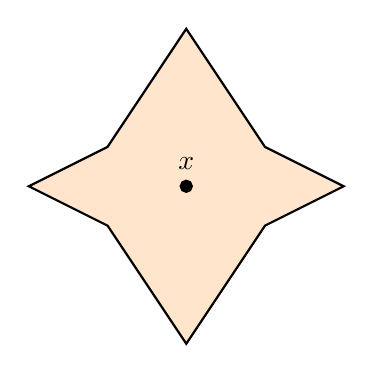
\begin{tikzpicture}[thick]
    \tikzstyle{point}=[circle,thick,draw=black,fill=black,inner sep=0pt,minimum width=4pt,minimum height=4pt]
    \draw[fill=orange!20] (-2,0) -- (-1,0.5) -- (0,2) -- (1,0.5) -- (2,0) -- (1,-0.5) -- (0,-2) -- (-1,-0.5) -- cycle;
    \node (a)[point,label=$x$] at (0,0) {};
\end{tikzpicture}

                \caption{Sternförmiges Gebiet}.
                \label{fig:sternfoermiges-gebiet}
            \end{figure}
        \item $\pi_1(S^2, x_0) = \Set{e}$, da im $\mdr^2$ alle Wege
              homotop zu $\Set{e}$ sind. Mithilfe der stereographischen
              Projektion kann von $S^2$ auf den $\mdr^2$ abgebildet
              werden.

              Dieses Argument funktioniert nicht mehr bei flächenfüllenden
              Wegen, d.~h. wenn $\gamma: I \rightarrow S^2$ surjektiv
              ist.
    \end{bspenum}
\end{beispiel}

\begin{bemerkung}\label{kor:gruppenisomorphismus-wege}
    Sei $X$ ein topologischer Raum, $a,b \in X$, $\delta: I \rightarrow X$
    ein Weg von $a$ nach $b$.

    Dann ist die Abbildung
    \[\alpha: \pi_1 (X, a) \rightarrow \pi_1(X,b)\;\;\;[\gamma] \mapsto [\overline{\delta} * \gamma * \delta]\]
    ein Gruppenisomorphismus.
\end{bemerkung}

\begin{figure}[htp]
    \centering
    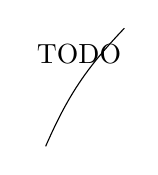
\begin{tikzpicture}
    \path (0,0)  edge [bend angle=10,bend right] node[label=TODO] {} (-1,-1.5);
\end{tikzpicture}

    \caption{Situation aus \cref{kor:gruppenisomorphismus-wege}}.
    \label{fig:situation-gruppenisomorphismus-wege}
\end{figure}

\begin{beweis}
    \begin{align*}
        \alpha([\gamma_1] * [\gamma_2]) &= [\overline{\delta} * (\gamma_1 * \gamma_2) * \delta]\\
        &= [\overline{\delta} * \gamma_1 * \delta * \overline{\delta} * \gamma_2 * \delta]
        &= [\overline{\delta} * \gamma_1 * \delta] * [\overline{\delta} * \gamma_2 * \delta]\\
        &= \alpha([\gamma_1]) * \alpha([\gamma_2])
    \end{align*}
\end{beweis}

%%%%%%%%%%%%%%%%%%%%%%%%%%%%%%%%%%%%%%%%%%%%%%%%%%%%%%%%%%%%%%%%%%%%%
% Tânias Mitschrieb vom 10.12.2013                                  %
%%%%%%%%%%%%%%%%%%%%%%%%%%%%%%%%%%%%%%%%%%%%%%%%%%%%%%%%%%%%%%%%%%%%%
\begin{definition}\xindex{einfach zusammenhängend}%11.4
    Ein wegzusammenhängender topologischer Raum $X$ heißt
    \textbf{einfach zusammenhängend}, wenn $\pi_1(X,x) = \Set{e}$
    für ein $x \in X$.
\end{definition}

Wenn $\pi_1(X,x) = \Set{e}$ für ein $x \in X$ gilt, dann wegen 
\cref{kor:gruppenisomorphismus-wege} sogar für alle $x \in X$.

\begin{bemerkung}\label{korr:11.5}
    Es seien $X, Y$ topologische Räume, $f:X \rightarrow Y$ eine
    stetige Abbildung, $x \in X, y := f(x) \in Y$.

    \begin{bemenum}
        \item Dann ist die Abbildung $f_* : \pi_1(X,x) \rightarrow \pi_1(Y, y),
        [\gamma] \rightarrow [f \circ \gamma]$ ein Gruppenhomomorphismus.
        \item Ist $Z$ ein weiterer topologischer Raum und $g: Y \rightarrow Z$
              eine stetige Abbildung $z:= g(y)$. Dann ist
              $(g \circ f)_* = g_* \circ f_*: \pi_1(X,x) \rightarrow \pi_1(Z,z)$
    \end{bemenum}
\end{bemerkung}

\begin{beweis}\leavevmode
    \begin{enumerate}[label=\alph*)]
        \item $f_*$ ist wohldefiniert: Seien $\gamma_1, \gamma_2$ homotope
              Wege von $x$. z.Z.: $f \circ \gamma_1 \sim f \circ \gamma_2$:
              Nach Voraussetzung gibt es stetige Abbildungen $H:I\times I \rightarrow X$
              mit 
              \begin{align*}
                H(t,0) &= \gamma_1(t),\\
                H(t,1) &= \gamma_2(t),\\
                H(0,s) &= H(1, s) = x\text{.}
              \end{align*}
              Dann ist $f \circ H: I \times I \rightarrow Y$ stetig mit
              $(f \circ H)(t,0) = f(H(t,0)) = f(\gamma_1(t)) = (f \circ \gamma_1)(t)$
              etc. $\Rightarrow f \circ \gamma_1 \sim f \circ \gamma_2$.

              $f_*([\gamma_1] * [\gamma_2]) = [f \circ (\gamma_1 * \gamma_2)] = [(f \circ \gamma_1)] * [(f \circ \gamma_2)] = f_*([\gamma_1]) * f_*([\gamma_2])$
        \item $(g \circ f)_* ([\gamma]) = [(g \circ f) \circ \gamma] = [g \circ (f \circ \gamma)] = g_* ([f \circ \gamma]) = g_* (f_* ([\gamma])) = (g_* \circ f_*)([\gamma])$
    \end{enumerate}
\end{beweis}

\begin{beispiel}
    \begin{bspenum}
        \item $f:S^1 \hookrightarrow \mdr^2$ ist injektiv, aber 
              $f_*:\pi_1(S^1, 1) \cong \mdz \rightarrow \pi_1(\mdr^2, 1) = \Set{e}$
              ist nicht injektiv
        \item $f: \mdr \rightarrow S^1, t \mapsto (\cos 2 \pi t, \sin 2 \pi t)$
              ist surjektiv, aber $f_*: \pi_1(\mdr, 0) = \Set{e} \rightarrow \pi_1(S^2, 1) \cong \mdz$
              ist nicht surjektiv
    \end{bspenum}
\end{beispiel}

\begin{bemerkung}%Folgerung 11.6
    Sei $f:X \rightarrow Y$ ein Homöomorphismus zwischen topologischen
    Räumen $X, Y$. Dann gilt:

    \[f_*: \pi_1(X,x) \rightarrow \pi_1(Y, f(x))\]
    ist ein Isomorphismus für jedes $x \in X$.
\end{bemerkung}

\begin{beweis}
    Sei $g: Y \rightarrow X$ die Umkehrabbildung, d.~h. $g$ ist stetig
    und $f \circ g = \id_Y$, $g \circ f = \id_X$

    $\Rightarrow f_* \circ g_* = (f \circ g)_* = (\id_Y)_* = \id_{\pi_1 (Y, f(X)}$
    und $g_* \circ f_* = \id_{\pi_1(X,x)}$.
\end{beweis}

\begin{definition}\xindex{Abbildung!homotope}
    Seien $X, Y$ topologische Räume, $x_0 \in X, y_0 \in Y, f, g: X \rightarrow Y$
    stetig mit $f(x_0) = y_0 = g(x_0)$.

    $f$ und $g$ heißen \textbf{homotop} ($f \sim g$), wenn es eine stetige
    Abbildung $H: X \times I \rightarrow Y$ gibt mit $H(x,0) = f(x), H(x,1)=g(x)$
    für alle $x \in X$ und $H(x_0, s) = y_0$ für alle $s \in I$.
\end{definition}

\begin{bemerkung}
    Sind $f$ und $g$ homotop, so ist $f_* = g_*: \pi_1 (X, x_0) \rightarrow \pi_1(Y, y_0)$.
\end{bemerkung}

\begin{beweis}
    Sei $\gamma$ ein geschlossener Weg in $X$ um $x_0$, d.~h.
    $[\gamma] \in \pi_1 (X, x_0)$.

    Z.~z.: $f \circ \gamma \sim g \circ \gamma$

    Sei dazu $H_\gamma: I \times I \rightarrow Y, (t,s) \mapsto H(\gamma(t), s)$.
    Dann gilt: 
        \begin{align*}
            H_\gamma(t,0) &= H(\gamma(t), 0) = (f \circ \gamma)(t) \;\forall t \in I\\
            H_\gamma(1,s) &= H(\gamma(1), s) = H(x_0, s) = y_0\;\forall s \in I\\
            H_\gamma(t,1) &= H(\gamma(t), 1) = g(\gamma(t))\;\forall t \in I
        \end{align*}
\end{beweis}

\begin{beispiel}
    $f:X \rightarrow Y, g: Y \rightarrow X$ mit $g \circ f \sim \id_X,$
    $f \circ g \sim \id_Y$

    $\Rightarrow f_*$ ist Isomorphismus. Konkret: $f: \mdr^2 \rightarrow \Set{0},$
    $g:\Set{0} \rightarrow \mdr^2$

    $\Rightarrow f \circ g = \id_{\Set{0}}$, $g \circ f: \mdr^2 \rightarrow \mdr^2$,
    $x \mapsto 0$ für alle $x$.

    $g \circ f \sim \id_{\mdr^2}$ mit Homotopie: $H: \mdr^2 \times I \rightarrow \mdr^2, H(x,s) = (1-s) x$ (stetig!)

    $\Rightarrow H(x,0) = x = \id_{\mdr^2} (x)$, $H(x, 1) = 0$, $H(0, s) = 0\;\forall s \in I$.
\end{beispiel}

\begin{satz}[Satz von Seifert und van Kampen \enquote{light}]\label{thm:seifert-van-kampen}
    Sei $X$ ein topologischer Raum, $U, V \subseteq X$ offen mit 
    $U \cup V = X$ und $U \cap V$ wegzusammenhängend.

    Dann wird $\pi_1(X,x)$ für $x \in U \cap V$ erzeugt von geschlossenen
    Wegen um $x$, die ganz in $U$ oder ganz in $V$ verlaufen.
\end{satz}

\begin{beweis}
    Sei $\gamma: I \rightarrow X$ ein geschlossener Weg um $x$.
    Überdecke $I$ mit endlich vielen offenen Intervallen
    $I_1, I_2, \dots, I_n$, die ganz in 
    $\gamma^{-1}(U)$ oder ganz in $\gamma^{-1}(V)$ liegen.

    \Obda sei $\gamma(I_1) \subseteq U, \gamma(I_2) \subseteq V$, etc.

    Wähle $t_i \in I_i \cap I_{i+1}$, also $\gamma(t_i) \in U \cap V$.
    Sei $\sigma_i$ Weg in $U \cap V$ von $x_0$ nach $\gamma(t_i) \Rightarrow \gamma$
    ist homotop zu 
    \[\underbrace{\gamma_1 * \overline{\sigma_1}}_{\text{in } U} * \underbrace{\sigma_1 * \gamma_2 * \overline{\sigma_2}}_{\text{in } V} * \dots * \sigma_{n-1} * \gamma_2\]
\end{beweis}

\begin{beispiel}
    \begin{bspenum}
        \item
            \begin{figure}[htp]
                \centering
                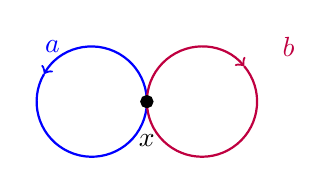
\begin{tikzpicture}[thick]
    \tikzstyle{point}=[circle,thick,draw=black,fill=black,inner sep=0pt,minimum width=4pt,minimum height=4pt]
    \node[blue]   at (4.5, 1.7) {$a$};
    \node[purple] at (7.5, 1.7) {$b$};
    \begin{scope}[xshift=5cm, yshift=1cm]
        \draw[blue,->]   (  0,0)+(150:0.7cm) arc (150:510:0.7cm);
        \draw[purple,<-] (1.4,0)+( 40:0.7cm) arc (40:400:0.7cm);
        \node (z)[point,label={[label distance=0.2cm]-90:$x$}] at (0.7,0) {};
    \end{scope}
\end{tikzpicture}

                \caption{Topologischer Raum $X$}
                \label{fig:top-raum-kreise}
            \end{figure}

            Sei $X$ wie in \cref{fig:top-raum-kreise}. $\pi_1(X,x)$ wird \enquote{frei} erzeugt von $a$ und $b$, weil
            $\pi_1(U,x) = <a> \cong \mdz, \pi_1(V,x) = <b> \cong \mdz$,
            insbesondere ist $a*b$ nicht homotop zu $b*a$.
        \item Torus: $\pi_1(T^2, X)$ wird erzeugt von $a$ und $b$.
            \begin{figure}[htp]
                \centering
                \documentclass[varwidth=true, border=2pt]{standalone}
\usepackage{tikz}
\usetikzlibrary{patterns}

\begin{document}
\begin{tikzpicture}[thick]
    \draw[pattern=north east lines] (-3,3) -- (3,3) -- (3,-3) -- (-3,-3) -- cycle;
    \draw[red, pattern color=red, pattern=north west lines] (-3,-1) -- (-1,-1) -- (-1,-3) -- (-3,-3) -- cycle;
    \draw[red, pattern color=red, pattern=north west lines] (-3,3) -- (-1,3) -- (-1,1) -- (-3,1) -- cycle;
    \draw[red, pattern color=red, pattern=north west lines] (1,3) -- (3,3) -- (3,1) -- (1,1) -- cycle;
    \draw[red, pattern color=red, pattern=north west lines] (1,-1) -- (3,-1) -- (3,-3) -- (1,-3) -- cycle;
    \draw[->,blue] (-3,-1.5) -- (-2,-1.5);
    \draw[blue] (-2,-1.5) -- (-1.5,-1.5);
    \draw[->,blue] (-1.5,-1.5) -- (-1.5,-2.3);
    \draw[blue] (-1.5, -2.3) -- (-1.5, -3);
    \draw[green] (-3,-2) -- (-2,-2) -- (-2, -3);
\end{tikzpicture}
\end{document}

                \caption{$a*b = b*a \Leftrightarrow a * b * \overline{a} * \overline{b} \sim e$}
                \label{fig:torous-a-b}
            \end{figure}
    \end{bspenum}
\end{beispiel}

%%%%%%%%%%%%%%%%%%%%%%%%%%%%%%%%%%%%%%%%%%%%%%%%%%%%%%%%%%%%%%%%%%%%%
% Mitschrieb vom 12.12.2013                                         %
%%%%%%%%%%%%%%%%%%%%%%%%%%%%%%%%%%%%%%%%%%%%%%%%%%%%%%%%%%%%%%%%%%%%%
\section{Überlagerungen}\index{Ueberlagerung@""Uberlagerung|(}
\begin{figure}[htp]
    \centering
    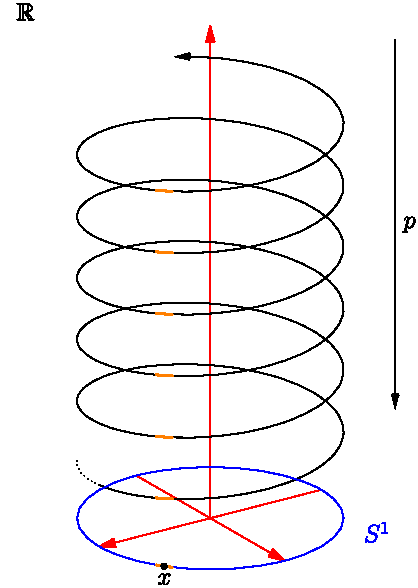
\includegraphics[width=4cm, keepaspectratio]{figures/topology-r-spiral-covering-s.pdf}
    \caption{$\mdr \rightarrow S^1$,\\$t \mapsto (\cos 2 \pi t, \sin 2 \pi t)$}
    \label{fig:ueberlappung-r1-spirale-s1}
\end{figure}
\begin{definition}\xindex{Ueberlagerung@""Uberlagerung}\label{def:12.1}%Definition 12.1 der Vorlesung
    Es seien $X, Y$ zusammenhängende topologische Räume und
    $p: Y \rightarrow X$ eine stetige Abbildung.

    $p$ heißt \textbf{Überlagerung}, wenn jedes $x \in X$ eine offene
    Umgebung $U = U(x) \subseteq X$ besitzt, sodass $p^{-1}(U)$ disjunkte Vereinigung
    von offenen Teilmengen $V_j \subseteq Y$ ist $(j \in I)$ und
    $p|_{V_j}: V_j \rightarrow U$ ein Homöomorphismus ist.
\end{definition}

\begin{beispiel}
    \begin{bspenum}
        \item siehe \cref{fig:ueberlappung-r1-spirale-s1}
        \item siehe \cref{fig:ueberlappung-kaestchen-torus}
        \item $\mdr^n \rightarrow T^n = \mdr^n / \mdz^n$
        \item $S^n \rightarrow \praum^n(\mdr)$\xindex{Raum!projektiver}
        \item $S^1 \rightarrow S^1$, $z \mapsto z^2$, siehe \cref{fig:liftung-s1-s1}
    \end{bspenum}

    \begin{figure}[htp]
        \centering
        \resizebox{0.95\linewidth}{!}{% The following answers were used to create this image:
% - http://tex.stackexchange.com/a/45824/5645 - Grid
% - http://tex.stackexchange.com/a/373/5645 - Torus
\documentclass[border=2pt]{standalone}
\usepackage{amsmath,amssymb}
\usepackage{tikz}
\usetikzlibrary{patterns,arrows,positioning}

\begin{document}
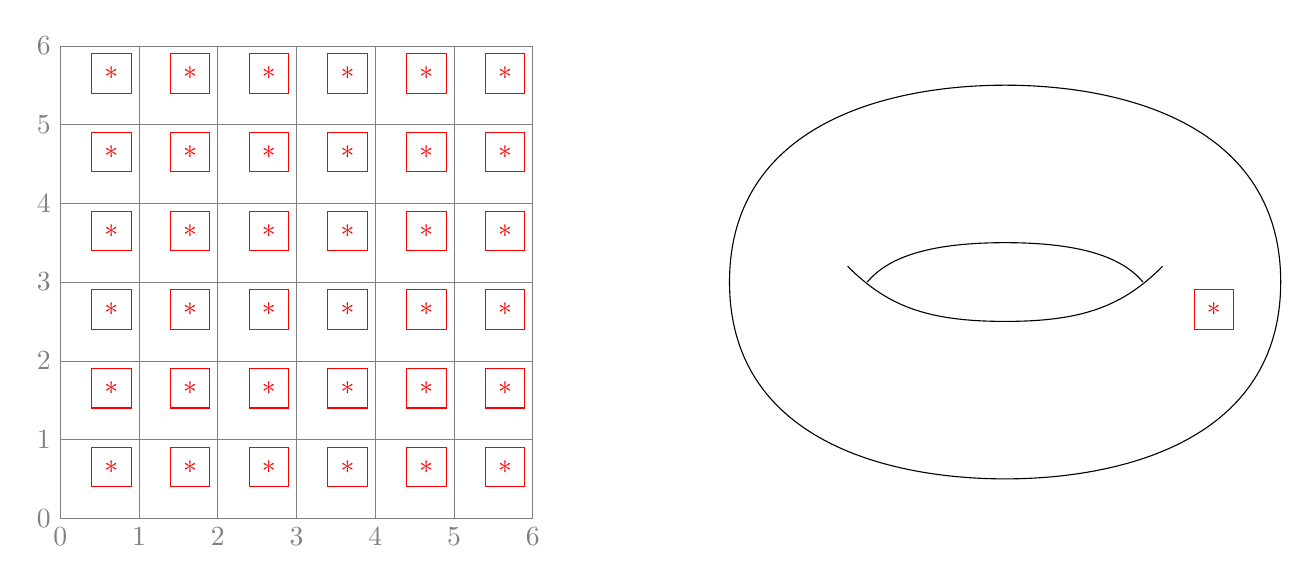
\begin{tikzpicture}
\tikzstyle{point}=[circle,thick,draw=black,fill=black,inner sep=0pt,minimum width=4pt,minimum height=4pt]
\newcommand*{\xMin}{0}%
\newcommand*{\xMax}{6}%
\newcommand*{\yMin}{0}%
\newcommand*{\yMax}{6}%

\draw (-3.5,0) .. controls (-3.5,2) and (-1.5,2.5) .. (0,2.5);
\draw[xscale=-1] (-3.5,0) .. controls (-3.5,2) and (-1.5,2.5) .. (0,2.5);
\draw[rotate=180] (-3.5,0) .. controls (-3.5,2) and (-1.5,2.5) .. (0,2.5);
\draw[yscale=-1] (-3.5,0) .. controls (-3.5,2) and (-1.5,2.5) .. (0,2.5);

\draw (-2,.2) .. controls (-1.5,-0.3) and (-1,-0.5) .. (0,-.5) .. controls (1,-0.5) and (1.5,-0.3) .. (2,0.2);
\draw (-1.75,0) .. controls (-1.5,0.3) and (-1,0.5) .. (0,.5) .. controls (1,0.5) and (1.5,0.3) .. (1.75,0);


\begin{scope}[shift={(-12,-3)}]
    \foreach \i in {\xMin,...,\xMax} {
        \draw [very thin,gray] (\i,\yMin) -- (\i,\yMax)  node [below] at (\i,\yMin) {$\i$};
    }
    \foreach \i in {\yMin,...,\yMax} {
        \draw [very thin,gray] (\xMin,\i) -- (\xMax,\i) node [left] at (\xMin,\i) {$\i$};
    }

    \begin{scope}[shift={(14,2)}]
        \node (P) at (0.4,0.9) {};
        \node (Q) at (0.9,0.4) {};
        \draw [red] (P) rectangle (Q);
        \draw (0.65, 0.6) node[red] {*};
    \end{scope}

    \foreach \x in {0,1,2,3,4,5} {
        \foreach \y in {0,1,2,3,4,5} {
            \begin{scope}[shift={(\x,\y)}]
                \node (P) at (0.4,0.9) {};
                \node (Q) at (0.9,0.4) {};
                \draw [red] (P) rectangle (Q);
                \draw (0.65, 0.6) node[red] {*};
            \end{scope}
        }
    }
\end{scope}
    \draw (-4.5, 0) node[below] {$\xrightarrow{\text{\;\;\;\;\;\;\;\;}}$};
\end{tikzpicture}
\end{document}
}
        \caption{$\mdr^2 \rightarrow T^2 = \mdr^2 / \mdz^2$}
        \label{fig:ueberlappung-kaestchen-torus}
    \end{figure}
    \begin{figure}[htp]
        \centering
        \newcommand\markangle[6]{% origin X Y radius radiusmark mark
  % fill red circle
  \begin{scope}
    \path[clip] (#1) -- (#2) -- (#3);
    \fill[color=red,fill opacity=0.5,draw=red,name path=circle]
    (#1) circle (#4);
  \end{scope}
  % middle calculation
  \path[name path=line one] (#1) -- (#2);
  \path[name path=line two] (#1) -- (#3);
  \path[%
  name intersections={of=line one and circle, by={inter one}},
  name intersections={of=line two and circle, by={inter two}}
  ] (inter one) -- (inter two) coordinate[pos=.5] (middle);
  % put mark
  \node at ($(#1)!#5!(middle)$) {#6};
}

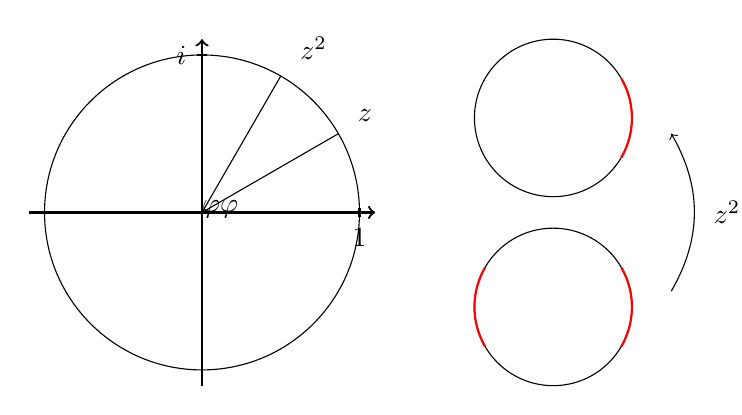
\begin{tikzpicture}
    \newcommand{\R}{2}
    \draw (0,0) circle (\R);
    \draw[->, thick] ({-(\R+0.2)},0) -- ({\R+0.2},0);
    \draw[->, thick] (0,{-(\R+0.2)}) -- (0,{\R+0.2});
    \draw[thick] (\R,-0.06) -- (\R,0.06) node[label=below:$1$] {};
    \draw[thick] (-0.06,\R) -- (0.06,\R) node[label=left:$i$] {};
    \draw (0,0) -- ({\R*cos(30)},{\R*sin(30)}) node[label=15:$z$] {};
    \draw (0,0) -- ({\R*cos(60)},{\R*sin(60)}) node[label=35:$z^2$] {};

    \coordinate (O) at (0,0);
    \coordinate (X) at (1,0);
    \coordinate (Y) at ({\R*cos(30)},{\R*sin(30)});
    \coordinate (Z) at ({\R*cos(60)},{\R*sin(60)});
    \markangle{O}{Y}{Z}{10mm}{7mm}{$\varphi$}
    \markangle{O}{X}{Y}{10mm}{7mm}{$\varphi$}

    \begin{scope}[xshift=4cm, yshift=-1.2cm]
        \draw (0,0) circle (\R/2);
        \newcommand{\x}{1}
        \draw [red,thick,domain=-30:30] plot ({cos(\x)}, {sin(\x)});
        \draw [red,thick,domain=210:150] plot ({cos(\x)}, {sin(\x)});
    \end{scope}

    \begin{scope}[xshift=4cm, yshift=+1.2cm]
        \draw (0,0) circle (\R/2);
        \newcommand{\x}{1}
        \draw [red,thick,domain=-30:30] plot ({cos(\x)}, {sin(\x)});
    \end{scope}

    \coordinate (T) at (5.5,1);
    \path[->] (5.5,-1) edge[bend right] node[label=right:$z^2$] {} (T);
\end{tikzpicture}

        \caption{$t \mapsto (\cos 4 \pi t, \sin 4 \pi t)$}
        \label{fig:liftung-s1-s1}
    \end{figure}
\end{beispiel}

\begin{bemerkung}
    Überlagerungen sind surjektiv.
\end{bemerkung}

\begin{beweis}
    Sei $p: Y \rightarrow X$ eine Überlagerung und $x \in X$ beliebig.
    Dann existiert eine offene Umgebung $U(x) \subseteq X$ und offene
    Teilmengen $V_j \subseteq X$ mit 
    $p^{-1}(U) = \Dcup V_j$ und
    $p|_{V_j}: V_j \rightarrow U$ ist Homöomorphismus.

    D.~h. es existiert ein $y \in V_j$, so dass $p|_{V_j}(y) = x$.
    Da $x \in X$ beliebig war und ein $y \in Y$ existiert, mit 
    $p(y) = x$, ist $p$ surjektiv.    $\qed$
\end{beweis}

\begin{definition}\xindex{Abbildung!offene}
    Seien $X, Y$ topologische Räume und $f:X \rightarrow Y$ eine 
    Abbildung.

    $f$ heißt \textbf{offen} $:\gdw \forall V \subseteq X$ offen: $f(V)$ ist offen in $Y$.
\end{definition}

\begin{bemerkung}\label{bem:12.2} % Bemerkung 12.2 der Vorlesung
    Überlagerungen sind offene Abbildungen.
\end{bemerkung}

\begin{beweis}
    Sei $y \in V$ und $x \in p(V)$, sodass $x=p(y)$ gilt.
    Sei weiter $U = U_x$ eine offene Umgebung von $x$ wie in \cref{def:12.1}
    und $V_j$ die Komponente von $p^{-1}(U)$, die $y$ enthält.

    Dann ist $V \cap V_j$ offene Umgebung von $y$.

    $\Rightarrow p(V \cap V_j)$ ist offen in $p(V_j)$, also auch offen
    in $X$. Außerdem ist $p(y) = x \in p(V \cap V_j)$ und
    $p(V \cap V_j) \subseteq p(V)$.

    $\Rightarrow p(V)$ ist offen.
\end{beweis}

\todo[inline]{Die Definition von Diskret habe ich mir überlegt. Hatten wir das schon mal? 
Haben wir Häufungspunkt definiert?}
\begin{definition}\xindex{diskret}
    Sei $X$ ein topologischer Raum und $M \subseteq X$.

    $M$ heißt \textbf{diskret} in $X$, wenn $M$ in $X$ keinen 
    Häufungspunkt hat.
\end{definition}

\begin{bemerkung} % Bemerkung 12.3 der Vorlesung
    Sei $p: Y \rightarrow X$ Überlagerung, $x \in X$.
    \begin{bemenum}
        \item $X$ hausdorffsch $\Rightarrow Y$ hausdorffsch
        \item $p^{-1}(x)$ ist diskret in $Y$ für jedes $x \in X$.
    \end{bemenum}
\end{bemerkung}

\begin{beweis}\leavevmode
    \begin{enumerate}[label=\alph*)]
        \item Seien $y_1, y_2 \in Y$.

        \underline{1. Fall}: $p(y_1) = p(y_2) = x$.

        Sei $U$ Umgebung von $x$ wie in \cref{def:12.1},
        $V_{j_1}$ bzw. $V_{j_2}$ die Komponente von $p^{-1}(U)$, die
        $y_1$ bzw. $y_2$ enthält.

        Dann ist $V_{j_1} \neq V_{j_2}$, weil beide ein Element aus $p^{-1}(x)$
        enthalten.

        $\Rightarrow V_{j_1} \cap V_{j_2} = \emptyset$ nach Voraussetzung.

        \underline{2. Fall}: $p(y_1) \neq p(y_2)$.
        
        Dann seien $U_1$ und $U_2$ disjunkte Umgebungen von $p(y_1)$
        und $p(y_2)$.

        $\Rightarrow p^{-1}(U_1)$ und $p^{-1}(U_2)$ sind disjunkte 
        Umgebungen von $y_1$ und $y_2$.

        \item Sei $y \in Y$

        \underline{1. Fall}: $y \in p^{-1}(x)$

        Finde $v_j$, sodass kein \dots 
        \todo[inline]{...}

        \underline{2. Fall}: $y \notin p^{-1}(x)$

        \todo[inline]{...}
    \end{enumerate}
\end{beweis}

\begin{bemerkung}\label{kor:12.4}%Bemerkung 12.4 der Vorlesung
    Sei $p: Y \rightarrow X$ Überlagerung, $x_1, x_2 \in X$.

    Dann ist $|p^{-1} (x_1)| = |p^{-1}(x_2)|$.\footnote{$|p^{-1} (x_1)| = \infty$ ist erlaubt!}
\end{bemerkung}

\begin{beweis}
    Sei $U$ Umgebung von $x_1$ wie in \cref{def:12.1}, $x \in U$.
    Dann enthält jedes $V_j, j \in I_X$ genau ein Element von
    $p^{-1}(x)$

    $\Rightarrow |p^{-1} (x)|$ ist konstant auf $U$

    $\xRightarrow{X \text{zhgd.}} |p^{-1}(x)|$  ist konstant auf $X$
\end{beweis}

\begin{definition}\xindex{Liftung}
    Sei $p: Y \rightarrow X$ Überlagerung, $Z$ ein weiterer topologischer
    Raum, $f:Z \rightarrow X$ stetig.

    Eine stetige Abbildung $\tilde{f}: Z \rightarrow Y$ heißt
    \textbf{Liftung} von $f$, wenn $p \circ \tilde{f} = f$ ist.
\end{definition}

\begin{figure}[htp]
    \centering
    \resizebox{0.95\linewidth}{!}{% The following answers were used to create this image:
% - http://tex.stackexchange.com/a/45824/5645 - Grid
% - http://tex.stackexchange.com/a/373/5645 - Torus
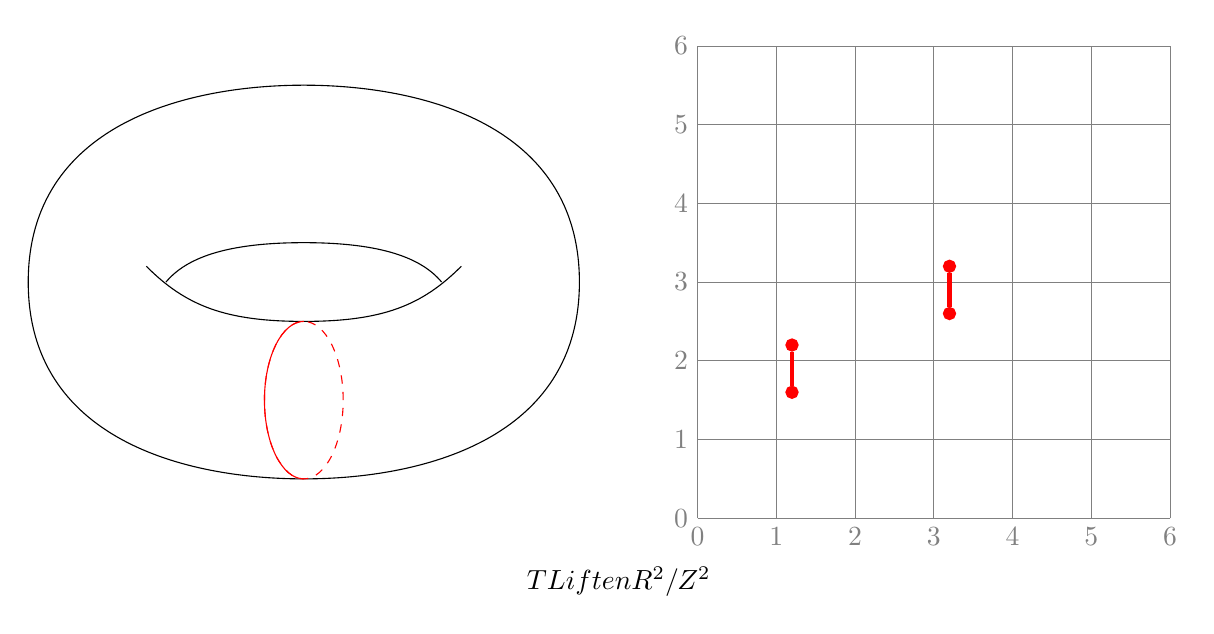
\begin{tikzpicture}
\tikzstyle{point}=[circle,thick,draw=black,fill=black,inner sep=0pt,minimum width=4pt,minimum height=4pt]
\newcommand*{\xMin}{0}%
\newcommand*{\xMax}{6}%
\newcommand*{\yMin}{0}%
\newcommand*{\yMax}{6}%

\draw (-3.5,0) .. controls (-3.5,2) and (-1.5,2.5) .. (0,2.5);
\draw[xscale=-1] (-3.5,0) .. controls (-3.5,2) and (-1.5,2.5) .. (0,2.5);
\draw[rotate=180] (-3.5,0) .. controls (-3.5,2) and (-1.5,2.5) .. (0,2.5);
\draw[yscale=-1] (-3.5,0) .. controls (-3.5,2) and (-1.5,2.5) .. (0,2.5);

\draw (-2,.2) .. controls (-1.5,-0.3) and (-1,-0.5) .. (0,-.5) .. controls (1,-0.5) and (1.5,-0.3) .. (2,0.2);

\draw (-1.75,0) .. controls (-1.5,0.3) and (-1,0.5) .. (0,.5) .. controls (1,0.5) and (1.5,0.3) .. (1.75,0);

\begin{scope}[shift={(5,-3)}]
    \foreach \i in {\xMin,...,\xMax} {
        \draw [very thin,gray] (\i,\yMin) -- (\i,\yMax)  node [below] at (\i,\yMin) {$\i$};
    }
    \foreach \i in {\yMin,...,\yMax} {
        \draw [very thin,gray] (\xMin,\i) -- (\xMax,\i) node [left] at (\xMin,\i) {$\i$};
    }

    \node (P)[point,red] at (1.2,2.2) {};
    \node (Q)[point,red] at (1.2,1.6) {};
    \draw[ultra thick, red] (P) -- (Q);

    \begin{scope}[shift={(2,1)}]
        \node (P)[point,red] at (1.2,2.2) {};
        \node (Q)[point,red] at (1.2,1.6) {};
        \draw[ultra thick, red] (P) -- (Q);
    \end{scope}
    \draw (-1, -0.5) node[below] {$T \xrightarrow{\text{Liften}} \mathbb{R}^2 / \mathbb{Z}^2$};
    \draw[red,dashed] (-5,1.5) ellipse (0.5cm and 1cm);

    \draw[red] (-5,2.5) arc (-270:-90:0.5 and 1) ;
\end{scope}
\end{tikzpicture}
}
    \caption{Beim Liften eines Weges bleiben geschlossene Wege im allgemeinen nicht geschlossen}
    \label{fig:satz-seifert-van-kampen}
\end{figure}

\begin{bemerkung}[Eindeutigkeit der Liftung]\label{kor:12.5}%Bemerkung 12.5 aus Vorlesung
    Sei $Z$ zusammenhängend und $f_0, f_1: Z \rightarrow Y$
    Liftungen von $f$.

    $\exists z_0 \in Z: f_0(z_0) = f_1(z_0) \Rightarrow f_0 = f_1$
\end{bemerkung}

\begin{figure}[htp]
    \centering
    \documentclass{article}
\usepackage[pdftex,active,tightpage]{preview}
\setlength\PreviewBorder{2mm}
\usepackage{tikz}

\begin{document}
\begin{preview}
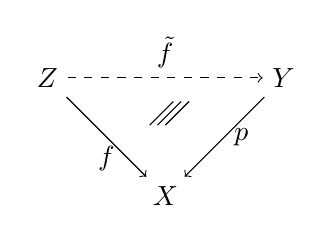
\begin{tikzpicture}
    \node (Z) at (0,0) {$Z$};
    \node (Y) at (3,0) {$Y$};
    \node (X) at (1.5,-1.5) {$X$};
    \draw[->, above, dashed] (Z) to node {$\tilde{f}$} (Y);
    \draw[->, below] (Z)  to node {$f$} (X);
    \draw[->, right] (Y)  to node {$p$} (X);

    \begin{scope}[xshift=1.3cm,yshift=-0.6cm]
        \draw (0,0) -- (0.3,0.3);
        \draw (0.1,0) -- (0.4,0.3);
        \draw (0.2,0) -- (0.5,0.3);
    \end{scope}
\end{tikzpicture}
\end{preview}
\end{document}

    \caption{Situation aus \cref{kor:12.5}}
    \label{fig:situation-kor-12.5}
\end{figure}

\begin{beweis}
    Sei $T = \Set{z \in Z | f_0(z) = f_1(z)}$.

    \underline{Z.~z.}: $T$ ist offen und $Z \setminus T$ ist auch offen.

    Sei $z \in T, x = f(z), U$ Umgebung von $x$ wie in \cref{def:12.1},
    $V$ die Komponente von $p^{-1}(U)$, die $y:=f_0(z) = f_1(z)$
    enthält.

    Sei $q:U \rightarrow V$ die Umkehrabbildung zu $p|_V$.

    Sei $W:= f^{-1}(U) \cap f_0^{-1}(V) \cap f_1^{-1}(V)$. $W$ ist 
    offene Umgebung in $Z$ von $z$.

    \underline{Behauptung:} $W \subseteq T$

    Denn für $w \in W$ ist $q(f(w)) = q((p \circ f_0))(w) = ((q \circ p) \circ f_0) (w) = f_0(w) = q(f(w)) = f_1(w)$

    $\Rightarrow T$ ist offen.

    Analog: $Z \setminus T$ ist offen.
\end{beweis}

\begin{satz}\label{thm:ueberlagerung-weg-satz-12.6}
    Sei $p: Y \rightarrow X$ Überlagerung, $\gamma: I \rightarrow X$
    ein Weg, $y \in Y$ mit $p(y) = \gamma(0) =: x$.

    Dann gibt es genau einen Weg $\tilde{\gamma}: I \rightarrow Y$
    mit $\tilde{\gamma}(0)=y$ und $p \circ \tilde{\gamma} = \gamma$.
\end{satz}

%%%%%%%%%%%%%%%%%%%%%%%%%%%%%%%%%%%%%%%%%%%%%%%%%%%%%%%%%%%%%%%%%%%%%
% Sebastians Mitschrieb vom 17.12.2013                              %
%%%%%%%%%%%%%%%%%%%%%%%%%%%%%%%%%%%%%%%%%%%%%%%%%%%%%%%%%%%%%%%%%%%%%
$p:Y \rightarrow X$ Überlagerung, $X,Y$ wegzusammenhängend.
$p$ stetig und surjektiv, zu $x \in X \exists$ Umgebung $U$, so dass
$p^{-1}(U) = \bigcup V_j$

$p|V_j: V_j \rightarrow U$ Homöomorphismus.

\begin{bemerkung}%Bemerkung 12.6 der Vorlesung
    Wege in $X$ lassen sich zu Wegen in $Y$ liften.

    Zu jedem $y \in p^{-1}(\gamma(0))$ gibt es genau einen Lift von 
    $\gamma$.
\end{bemerkung}

\begin{proposition}\label{proposition:12.7}%Proposition 12.7 der Vorlesung
    Seien $p: Y \rightarrow X$ eine Überlagerung, $a,b \in X$,
    $\gamma_0, \gamma_1: I \rightarrow X$ homotope Wege von $a$ nach
    $b$, $\tilde{a} \in p^{-1}(a), \tilde{\gamma_0}, \tilde{\gamma_1}$
    Liftungen von $\gamma_0$ bzw. $\gamma_1$ mit 
    $\tilde{\gamma_i}(0) = \tilde{a}$.

    Dann ist $\tilde{\gamma_0}(1) = \tilde{\gamma_1}(1)$ und
    $\tilde{\gamma_0} \sim \tilde{\gamma_1}$.
\end{proposition}

\begin{beweis}
    Sei $H: I \times I \rightarrow X$ Homotopie zwischen $\gamma_1$
    und $\gamma_2$.

    Für $s \in [0,1]$ sei $\gamma_s: I \rightarrow X$, $t \mapsto H(t,s)$.

    Sei $\tilde{\gamma_s}$ Lift von $\gamma_s$ mit $\tilde{\gamma_s}(0) = \tilde{a}$

    Sei $\tilde{H}: I \times I \rightarrow Y,\;\;\; \tilde{H}(t,s) := (\tilde{\gamma_s}(t), s)$

    Dann gilt:
    \begin{enumerate}[label=(\roman*)]
        \item $\tilde{H}$ ist stetig (Beweis wie für \cref{kor:12.5})
        \item $\tilde{H}(t,0) = \tilde{\gamma_0}(t) = \tilde{H}(t,1) = \tilde{\gamma_1}(t)$
        \item $\tilde{H}(0,s) = \tilde{\gamma_s}(0) = \tilde{a}$
        \item $\tilde{H}(1,s) \in p^{-1}(b)$
    \end{enumerate}

    Da $p^{-1}(b)$ diskrete Teilmenge von $Y$ ist\\
    $\Rightarrow \tilde{b_s} = \tilde{H}(1,s) = \tilde{H}(1,0) \;\forall s \in I$\\
    $\Rightarrow \tilde{b_0} = \tilde{b_1}$ und $\tilde{H}$ ist Homotopie 
    zwischen $\tilde{\gamma_0}$ und $\tilde{\gamma_1}$. $\qed$
\end{beweis}

\begin{folgerung}%In Vorlesung: "Folgerung 12.8"
    Sei $p: Y \rightarrow X$ eine Überlagerung, $x_0 \in X, y_0 \in p^{-1}(x_0)$
    \begin{bemenum}
        \item \label{folg:12.8a} $p_1: \pi_1(Y, y_0) \rightarrow \pi_1(X, x_0)$ ist injektiv\label{kor:12.8a}
        \item \label{folg:12.8b} $[\pi_1(X, x_0): p_* (\pi_1(Y, y_0))] = \deg(p)$\label{kor:12.8b}
    \end{bemenum}
\end{folgerung}

\begin{beweis}\leavevmode
    \begin{enumerate}[label=\alph*)]
        \item Sei $\tilde{\gamma}$ ein Weg in $Y$ um $y_0$ und
              $p_* ([\tilde{\gamma}]) = e$, also $p \circ \tilde{\gamma} \sim \gamma_{x_0}$

              Nach \cref{proposition:12.7} ist dann 
              $\tilde{\gamma}$ homotop zum Lift des konstanten Wegs
              $\gamma_{x_0}$ mit Anfangspunkt $y_0$, also zu
              $\gamma_{y_0} \Rightarrow [\tilde{\gamma}] = e$
        \item Sei $d = \deg{p}, p^{-1}(x_0) = \Set{y_0, y_1, \dots, y_{d-1}}$.
              Für einen geschlossenen Weg $\gamma$ in $X$ um $x_0$
              sei $\tilde{\gamma}$ die Liftung mit $\tilde{\gamma}(0) = y_0$.

              $\tilde{\gamma}(1) \in \Set{y_0, \dots, y_{d-1}}$ hängt
              nur von $[\gamma] \in \pi_1(X,x_0)$ ab.

              Für geschlossene Wege $\gamma_0, \gamma_1$ um $x$ gilt:

              \begin{align*}
                \tilde{\gamma_0}(1) &= \tilde{\gamma_1}(1)\\
                \Leftrightarrow [\tilde{\gamma_0} * \tilde{\gamma_1}^{-1}] &\in \pi_1(Y, y_0)\\
                \Leftrightarrow [\gamma_0 * \gamma_1^{-1}] &\in p_* (\pi_1(Y,y_0))\\
                \Leftrightarrow [\gamma_0] \text{ und } [\gamma_1] &\text{liegen in der selben Nebenklasse bzgl.} p_*(\pi_1(Y, y_0))
              \end{align*}

              Zu $i \in \Set{0, \dots, d-1}$ gibt es Weg $\delta_i$ in
              $Y$ mit $\delta_i(0) = y_0$ und $\delta_i(1) = y_i$\\
              $\Rightarrow p \cup \delta_i$ ist geschlossener Weg in 
              $X$ um $x_0$.\\
              $\Rightarrow$ Jedes $y_i$ mit $i=0, \dots, d-1$ ist 
              $\tilde{\gamma}(1)$ für ein $[\gamma] \in \pi_1(X,x_0)$.
    \end{enumerate}
\end{beweis}

\begin{bemerkung}%In Vorlesung: "Folgerung 12.9"
    Sei $p: Y \rightarrow X$ Überlagerung und $X$ einfach zusammenhängend.

    Dann ist $p$ ein Homöomorphismus.
\end{bemerkung}

\begin{beweis}
    Wegen \cref{folg:12.8a} ist auch $Y$ einfach zusammenhängend
    und wegen \cref{folg:12.8b} ist $\deg(p)=1$, $p$ ist also
    bijektiv.

    Nach \cref{bem:12.2} ist $p$ offen $\Rightarrow p^{-1}$
    ist stetig. $\Rightarrow p$ ist Homöomorphismus.  $\qed$
\end{beweis}

\begin{definition}%In Vorlesung: "Definition 12.10"
    Eine Überlagerung $p: \tilde{X} \rightarrow X$ heißt
    \textbf{universell}\xindex{Ueberlagerung@""Uberlagerung!universelle}, wenn
    $\tilde{X}$ einfach zusammenhängend ist.
\end{definition}

\begin{beispiel}
    $\mdr \rightarrow S^1, \;\;\; t \mapsto (\cos 2 \pi t, \sin 2 \pi t)$

    $\mdr^2 \rightarrow T^2 = \mdr^2 / \mdz^2$

    $S^n \rightarrow \praum^n(\mdr)$ für $n \geq 2$
\end{beispiel}

\begin{satz}\label{thm:12.11}%In Vorlesung: Satz 12.11
    Sei $p: \tilde{X} \rightarrow X$ eine universelle Überlagerung,
    $q:Y \rightarrow X$ weitere Überlagerung.

    Sei $x_0 \in X, \tilde{x_0} \in \tilde{X}, y_0 \in Y$ mit
    $q(y_1) = x_0, p(\tilde{x_0}) = x_0$.

    Dann gibt es genau eine Überlagerung $\tilde{p}: \tilde{X} \rightarrow Y$
    mit $\tilde{p}(\tilde{x_0}) = y_0$.
\end{satz}

\begin{beweis}
    Sei $z \in \tilde{X}, y_z: I \rightarrow \tilde{X}$ ein Weg von
    $\tilde{x_0}$ nach $z$.

    Sei $\delta_Z$ die eindeutige Liftung von $p \circ \gamma_z$
    nach $y$ mit $\delta_2(0) = y_0$.

    Setze $\tilde{p}(z) = \delta_Z(1)$.

    Da $\tilde{X}$ einfach zusammenhängend ist, hängt $\tilde{p}(z)$
    nicht vom gewählten $y_z$ ab.

    Offensichtlich ist $q(\tilde{p}(z)) = p(z)$.

    $\tilde{p}$ ist stetig (in $z \in \tilde{X}$). Sei $W \subseteq Y$
    offene Umgebung von $\tilde{p}(z)$.

    $\xRightarrow{q \text{ offen}} q(W)$ ist offene Umgebung von $p(z) \cdot d(\tilde{p}(z))$.

    Sei $U \subseteq q(W)$ offen wie in \cref{def:12.1} und
    $V \subseteq q^{-1}(U)$ die Komponente, die $\tilde{p}(z)$
    enthält.

    \Obda sei $V \subseteq W$.

    Sei $Z := p^{-1}(U)$. Für $u \in Z$ sei $\delta$ ein Weg in $Z$
    von $z$ nach $u$.

    $\Rightarrow \gamma_Z * \delta$ ist Weg von $x_0$ nach $u$\\
    $\Rightarrow \tilde{p}(u) \in V$\\
    $\Rightarrow Z \subseteq \tilde{p^{-1}}(W)$\\
    $\Rightarrow \tilde{p}$ ist stetig
\end{beweis}

%%%%%%%%%%%%%%%%%%%%%%%%%%%%%%%%%%%%%%%%%%%%%%%%%%%%%%%%%%%%%%%%%%%%%
% Mitschrieb vom 19.12.2013                                         %
%%%%%%%%%%%%%%%%%%%%%%%%%%%%%%%%%%%%%%%%%%%%%%%%%%%%%%%%%%%%%%%%%%%%%
\begin{bemerkung}%Vorlesung: Folgerung 12.12
    \todo{Hier stimmt was mit den Tilden nicht}
    Sind $p:X \rightarrow X$ und $y: \tilde{Y} \rightarrow X$
    universelle Überlagerungen, so sind $\tilde{X}$ und $\tilde{Y}$
    homöomorph.
\end{bemerkung}

\begin{beweis}
    Seien $x_0 \in X, \tilde{x_0} \in \tilde{X}$ mit 
    $p(\tilde{x_0}) = x_0$ und 
    $\tilde{y_0} \in q^{-1}(x_0) \subseteq \tilde{Y}$.

    Nach \cref{thm:12.11} gibt es genau eine Überlagerung
    \[f:\tilde{X} \rightarrow \tilde{Y} \text{ mit } f(x_0) = \tilde{Y_0} \text{ und } q \circ f = p\]
    und genau eine Überlagerung
    \[g: \tilde{Y} \rightarrow \tilde{X} \text{ mit } g(\tilde{y_0}) = \tilde{x_0} \text{ und } p \circ g = q\]

    Damit gilt: $p \circ q \circ f = q \circ f = p$, $q \circ f \circ g = p \circ g = q$.
    Also ist $g \circ f: \tilde{X} \rightarrow \tilde{X}$ Lift von 
    $p:\tilde{X} \rightarrow X$ mit $(g \circ f) (\tilde{x_0}) = \tilde{x_0}$.

    Da auch $\id_{\tilde{x}}$ diese Eigenschaft hat, folgt mit
    \cref{kor:12.4}: $g \circ f = \id_{\tilde{X}}$.
    Analog $f \circ g = \id_{\tilde{Y}}$. $\qed$
\end{beweis}

Die Frage, wann es eine universelle Überlagerung gibt, beantwortet
der folgende Satz:

\begin{satz}%In Vorlesung: Satz 12.13
    Es sei $X$ ein wegzusammenhängender topologischer Raum in dem
    jeder Punkt eine Umgebungsbasis aus einfach zusammenhängenden
    Mengen hat.

    Dann gibt es eine universelle Überlagerung.
\end{satz}

\begin{beweis}
    Sei $x_0 \in X$ und $\tilde{X} := \Set{(x, [\gamma]) | x \in X, \gamma \text{ Weg von } x_o \text{ nach } x}$
    und $p: \tilde{X} \rightarrow X, (x, [\gamma]) \mapsto x$.

    Die Topologie auf $\tilde{X}$ ist folgende:
    Definiere eine Umgebungsbasis von $(x, [\gamma])$ wie folgt:
    Es sei $U$ eine einfach zusammenhängende Umgebung von $x$ und
    \[\tilde{U} = \tilde{U}(x, [\gamma]) := \Set{(y, [\gamma * \alpha]) | y \in U, \alpha \text{ Weg in } U \text{ von } x \text{ nach } y} \]

    $p$ ist Überlagerung: $p|_{\tilde{U}} : \tilde{U} \rightarrow U$
    bijektiv. $p$ ist stetig und damit $p|_{\tilde{U}}$ ein 
    Homöomorphismus.

    Sind $\gamma_1, \gamma_2$ Wege von $x_0$ nach $x$ und $\gamma_1 \sim \gamma_2$,
    so ist $\tilde{U}(x, [\gamma_1]) \cap \tilde{U}(x, [\gamma_2]) = \emptyset$,
    denn: Ist $\gamma_1 * \alpha \sim \gamma_2 * \alpha$, so ist auch
    $\gamma_1 \sim \gamma_2$. Also ist $p$ eine Überlagerung.

    $\tilde{X}$ ist einfach zusammenhängend: Es sei $\tilde{x_0} := (x_0, e)$
    und $\tilde{\gamma}: I \rightarrow \tilde{X}$ ein geschlossener
    Weg um $\tilde{x_0}$.

    Sei $\gamma := p(\tilde{\gamma})$.

    \underline{Annahme}: $[\tilde{\gamma}] \neq e$

    Mit \cref{kor:12.8a} folgt dann: $[\gamma] \neq e$.

    Dann ist der Lift von $\gamma$ nach $\tilde{x}$ mit Anfangspunkt
    $\tilde{x_0}$ ein Weg von $\tilde{x_0}$ nach $(x_0, [\gamma])$.
    Widerspruch.
\end{beweis}

\begin{definition}\xindex{Decktransformation}%In Vorlesung: Def+Bem 12.14
    Es sei $p:Y \rightarrow X$ eine Überlagerung und $f:Y \rightarrow Y$
    ein Homöomorphismus.

    $f$ heißt \textbf{Decktransformation} von $p :\gdw p \circ f = p$.

    Ist $p$ eine Decktransformation und $|\Deck(Y/X)| = \deg{p}$,
    so heißt $p$ \textbf{regulär}.\xindex{Decktransformation!reguläre}
\end{definition}

\begin{bemerkung}%In Vorlesung:12.14
    \begin{bemenum}
        \item Die Decktransformationen von $p$ bilden eine Gruppe, 
              die sog. \textbf{Decktransformationsgruppe}\xindex{Decktransformationsgruppe}
              $\Deck(p) = \Deck(Y/X) = \Deck(Y \rightarrow X)$
        \item Ist $f \in \Deck(Y/X)$ und $f \neq \id$, dann hat
              $f$ keinen Fixpunkt.
        \item $|\Deck(Y/X)| \leq \deg{p}$\label{kor:12.14c}
        \item Ist $p$ eine reguläre Decktransformation, dann gilt:
              $\forall x \in X: \Deck(Y/X)$ operiert transitiv
              auf der Menge der Urbilder $p^{-1}(x)$.
    \end{bemenum}
\end{bemerkung}

\begin{beweis}\leavevmode
    \begin{enumerate}[label=\alph*)]
        \item Es gilt:
            \begin{itemize}
                \item $\id_Y \in \Deck{Y/X}$,
                \item $f,g \in \Deck{Y/X} \Rightarrow p \circ (f \circ g) = (p \circ f) \circ g = p \circ g \Rightarrow f \circ g \in \Deck{Y/X}$
                \item $f \in \Deck{Y/X} \Rightarrow p \circ f =$
                      $p \Rightarrow p \circ f^{-1} =$
                      $(p \circ f) \circ f^{-1} =$
                      $p \circ (f \circ f^{-1}) = p \Rightarrow f^{-1} \in \Deck{Y/X}$
            \end{itemize}
        \item Die Menge
              \[\Fix(f) = \Set{y \in Y | f(y) = y}\]
              ist abgeschlossen als Urbild der Diagonale 
              $\Delta \subseteq Y \times Y$ unter der stetigen
              Abbildung $y \mapsto (f(y),y)$. Außerdem ist $\Fix(f)$
              offen, denn ist $y \in \Fix(f)$, so sei $U$ eine 
              Umgebung von $p(y) \in X$ wie in \cref{def:12.1}
              und $U \subseteq p^{-1}(U)$ die Komponente, die $y$
              enthält; also $p:V \rightarrow U$ ein Homöomorphismus.
              Dann ist $W := f^{-1}(V) \cap V$ offene Umgebung von $y$.

              Für $z \in W$ ist $f(z) \in V$ und $p(f(z)) = p(z)$.
              Da $p$ injektiv auf $V$ ist, folgt $f(z) = z$, d.~h.
              $\Fix(f) \neq \emptyset$.

              Da $Y$ zusammenhängend ist, folgt aus $\Fix(\tilde{f}) \neq \emptyset$
              schon $\Fix(f) = Y$, also $f = \id_Y$.
        \item Es sei $x_0 \in X$, $\deg(p) = d$ und $p^{-1}(x_0) = \Set{y_0, \dots, y_{d-1}}$.
              Für $f \in \Deck(Y/X)$ ist $f(y_0)= \Set{y_0, \dots, y_{d-1}}$.

              Zu $i \in \Set{0, \dots, d-1}$ gibt es höchstens ein 
              $f \in \Deck(Y/X)$ mit $f(y_0) = y_1$, denn ist
              $f(y_0) = g(y_0)$, so ist \todo{Was steht hier?}{$(g^{-1} - f) y_0 = y_0$},
              also nach \cref{kor:12.14c} $g^{-1} \circ f = \id_Y$.
    \end{enumerate}
\end{beweis}

\begin{beispiel}
    \begin{bspenum}
        \item $p: \mdr \rightarrow S^1: \Deck(\mdr / S^1) = \Set{t \mapsto t + n | n \in \mdz} \cong \mdz$
        \item $p: \mdr^2 \rightarrow T^2: \Deck(\mdr^2 / T^2) \cong \mdz \times \mdz = \mdz^2$
        \item $p: S^n \rightarrow \praum^n(\mdr): \Deck(g^n / \praum^n(\mdr)) = \Set{x \mapsto \pm x} \cong \mdz / 2 \mdz$
    \end{bspenum}
\end{beispiel}

Nun werden wir eine Verbindung zwischen der Decktransformationsgruppe
und der Fundamentalgruppe herstellen:

\begin{satz}\label{thm:12.15}%In Vorlesung: Satz 12.15
    Ist $p: \tilde{X} \rightarrow X$ eine universelle Überlagerung, 
    so gilt:
    \[\Deck(\tilde{X}/X) \cong \pi_1(X, x_0)\;\;\;\forall x_0 \in X\]
\end{satz}

\begin{beweis}
    Wähle $\tilde{x_0} \in p^{-1}(x_0)$. Es sei $\rho: \Deck(\tilde{x}/x) \rightarrow \pi_1(X, x_0)$
    die Abbildung, die $f$ auf $[p(\gamma_f)]$ abbildet, wobei $\gamma_f$
    ein Weg von $\tilde{x_0}$ nach $f(\tilde{x_0})$ sei. Da $\tilde{x}$
    einfach zusammenhängend ist, ist $\gamma_f$ bis auf Homotopie
    eindeutig bestimmt und damit auch $\rho$ wohldefiniert.

    \begin{itemize}
        \item \underline{$\rho$ ist Gruppenhomomorphismus}: Seien 
            $f, g \in \Deck(\tilde{X}/ X) \Rightarrow \gamma_{g \circ f} = \gamma_g * g(\gamma_f)$
            $\Rightarrow p(\gamma_{g \circ f}) = p(\gamma_g) * \underbrace{(p \circ g)}_{=p} (\gamma_f) = \rho(g) \neq \rho(f)$
        \item \underline{$\rho$ ist injektiv}: $\rho(f) = e \Rightarrow p (\gamma_f) \sim \gamma_{x_0}$
            $\xRightarrow{\cref{thm:ueberlagerung-weg-satz-12.6}} \gamma_f \sim \gamma_{\tilde{x_0}}$ 
            $\Rightarrow f(x_0) = \tilde{x_0} \xRightarrow{\crefabbr{kor:12.14c}} f = \id_{\tilde{x}}$.
        \item \underline{$\rho$ ist surjektiv}: Sei $[\gamma] \in \pi_1(X, x_0)$,
            $\tilde{\gamma}$ Lift von $\gamma$ nach $\tilde{x}$ mit
            Anfangspunkt $\tilde{x_0}$. Der Endpunkt von $\tilde{\gamma}$
            sei $\tilde{x_1}$.

            \underline{$p$ ist reguläre Überlagerung}: Seien
            $\tilde{x_0}, \tilde{x_1} \in \tilde{X}$ mit 
            $p(\tilde{x_0}) = p(\tilde{x_1})$. Nach \cref{thm:12.11}
            gibt es genau eine Überlagerung $\tilde{p}: \tilde{X} \rightarrow X$
            mit $p=p \circ \tilde{p}$ und $\tilde{p}(\tilde{x_0}) = \tilde{x_1}$.
            Somit ist $\tilde{p}$ eine Decktransformation und damit
            $p$ eine reguläre Überlagerung.

            Da $p$ reguläre Überlagerung ist, gibt es ein $f \in \Deck(\tilde{X}/X)$
            mit $f(\tilde{x_0}) = \tilde{x_1}$.

            Aus der Definition von $\rho$ folgt: $\rho(f) = p (\gamma_f) = \gamma$
    \end{itemize}
            $\qed$
\end{beweis}

\begin{beispiel}[Bestimmung von $\pi_1(S^1)$]
    $p: \mdr \rightarrow S^1$, $t \mapsto (\cos 2 \pi t, \sin 2 \pi t)$
    ist universelle Überlagerung, da $\mdr$ zusammenhängend ist.

    Für $n \in \mdz$ sei $f_n: \mdr \rightarrow \mdr, t \mapsto t + n$
    die Translation um $n$.

    Es gilt: $(p \circ f_n)(t) = p(f_n(t)) = p(t) \;\;\; \forall t \in \mdr$,
    d.~h. $f_n$ ist Decktransformation.

    Ist umgekehrt $g$ irgendeine Decktransformation, so gilt insbesondere
    für $t=0$:
    \[(\cos(2 \pi g(0)), \sin(2 \pi g(0))) = (p \circ g)(0) = p(0) = (1,0)\]

    Es existiert $n \in \mdz$ mit $g(0) = n$. Da auch $f_n(0) = 0 + n = n$
    gilt, folgt mit \cref{kor:12.14c} $g = f_n$. Damit folgt:
    \[\Deck(\mdr/S^1) = \Set{f_n | n \in \mdz} \cong \mdz\]
    Nach \cref{thm:12.15} also $\pi_1(S^1) \cong \Deck(\mdr/S^1) \cong \mdz$
\end{beispiel}
\index{Ueberlagerung@""Uberlagerung|)}

%%%%%%%%%%%%%%%%%%%%%%%%%%%%%%%%%%%%%%%%%%%%%%%%%%%%%%%%%%%%%%%%%%%%%
% Lea's Mitschrieb vom 07.01.2014                                   %
%%%%%%%%%%%%%%%%%%%%%%%%%%%%%%%%%%%%%%%%%%%%%%%%%%%%%%%%%%%%%%%%%%%%%
\section{Gruppenoperationen}\index{Gruppenoperation|(}\index{Aktion|see{Gruppenoperation}}\index{Gruppenaktion|see{Gruppenoperation}}
\begin{definition}\xindex{Gruppenoperation}% in Vorlesung: Definition 13.1
    Sei $(G, \cdot)$ eine Gruppe und $X$ eine Menge.

    Eine \textbf{Gruppenoperation} von $G$ auf
    $X$ ist eine Abbildung $\circ$:
    
    \[ \circ: G \times X \rightarrow X,\;\;\; (g,x) \mapsto g \cdot x,\]

    für die gilt:
    \begin{defenum}
        \item $1_G \circ x = x \;\;\; \forall x \in X$\label{def:gruppenoperation.1}
        \item $(g \cdot h) \circ x = g \circ (h \circ x) \;\;\; \forall g,h \in G \forall x \in X$\label{def:gruppenoperation.2}
    \end{defenum}
\end{definition}

\begin{beispiel}
    \begin{enumerate}[label=\arabic*),ref=\thebeispiel.\arabic*]
        \item $G = (\mdz, +), X = \mdr, nx = x + n$\label{bsp:gruppenoperation1}
        \item $G$ operiert auf $X = G$ durch $g \circ h := g \cdot h$
        \item $G$ operiert auf $X = G$ durch $g \circ h := g \cdot h \cdot g^{-1}$, denn
        \begin{enumerate}[label=\roman*)]
            \item $1_G \circ h = 1_G \cdot h \cdot 1_G^{-1} = h$
            \item \begin{align*}
                    (g_1 \cdot g_2) \circ h &= (g_1 \cdot g_2) \cdot h \cdot (g \cdot g_2)^{-1}\\
                        &= g_1 \cdot (g_2 \cdot h \cdot g_2^{-1}) \cdot g_1^{-1}\\
                        &= g_1 \circ (g_2 \circ h)
                  \end{align*}
        \end{enumerate}
    \end{enumerate}
\end{beispiel}

\begin{definition}
    Sei $G$ eine Gruppe, $X$ ein topologischer Raum und
    $\circ: G \times X \rightarrow X$ eine Gruppenoperation.

    \begin{defenum}
        \item $G$ operiert durch Homomorphismen, wenn für jedes $g \in G$
              die Abbildung
              \[m_g: X \rightarrow X, x \mapsto g \cdot X\]
              ein Homöomorphismus ist.
        \item Ist $G$ eine topologische Gruppe, so heißt die Gruppenoperation $\circ$
              \textbf{stetig}\xindex{Gruppenoperation!stetige}, wenn 
              $\circ: G \times X \rightarrow X$ stetig ist.
    \end{defenum}
\end{definition}

\begin{bemerkung}%In Vorlesung: Bemerkung 13.2
     Jede stetige Gruppenoperation ist eine Gruppenoperation durch Homöomorphismen.
\end{bemerkung}
\begin{beweis}
    Nach Voraussetzung ist $\circ |_{\Set{g} \times X} : X \rightarrow X, x \mapsto g \circ x$ stetig.

    Die Umkehrabbildung zu $m_g$ ist $m_{g^{-1}}$: 
    \begin{align*}
        (m_{g^{-1}} \circ m_g)(x) &= m_{g^{-1}} (m_g (x))\\
            &= m_{g^{-1}} (g \circ x)\\
            &= g^{-1} \circ (g \circ x)\\
            &\overset{\mathclap{\crefabbr{def:gruppenoperation.2}}}{=} (g^{-1} \cdot g) \circ x\\
            &= 1_G \circ x\\
            &\overset{\mathclap{\crefabbr{def:gruppenoperation.1}}}{=} x
    \end{align*}
\end{beweis}

\begin{beispiel}
    In Beispiel~\ref{bsp:gruppenoperation1} operiert $\mdz$ durch Homöomorphismen.
\end{beispiel}

\begin{bemerkung}\label{kor:13.3}%In Vorlesung: Bemerkung 13.3
    Sei $G$ eine Gruppe und $X$ eine Menge.

    \begin{bemenum}
        \item Die Gruppenoperation von $G$ auf $X$ entsprechen bijektiv
              den Gruppenhomomorphismen $\varrho: G \rightarrow \Perm(X) = \Sym(X) = \Set{f: X \rightarrow X | f \text{ ist bijektiv}}$
        \item Ist $X$ ein topologischer Raum, so entsprechen dabei 
              die Gruppenoperationen durch Homöomorphismus den Gruppenhomomorphismen
              $G \rightarrow \Homoo(X)$
    \end{bemenum}
\end{bemerkung}

\begin{beweis}
    \item Sei $\circ: G \times X \rightarrow X$ eine Gruppenoperation von $G$
          auf $X$. Dann sei $\varrho: G \rightarrow \Perm(X)$ definiert
          durch $\varrho(g)(X) = g \cdot x \;\;\; \forall g \in G, x \in X$,
          also $\varrho(g) = m_g$.

          $\varrho$ ist Homomorphismus: $\varrho(g_1 \cdot g_2) = m_{g_1 \cdot g_2} = m_{g_1} \circ m_{g_2} = \varrho(g_1) \circ \varrho(g_2)$,
          denn für $x \in X: \varrho(g_1 \cdot g_2) (x) = (g_1 \cdot g_2) \circ x = g_1 \circ (g_2 \circ x) = \varrho(g_1) (\varrho(g_2)(x)) = (\varrho(g_1) \circ \varrho (g_2)) (x)$

          Umgekehrt: Sei $\varrho: G \rightarrow \Perm(X)$ Gruppenhomomorphismus. Definiere $\circ: G \times X \rightarrow X$ durch $g \circ x = \varrho (g)(x)$.

          z.~z. \cref{def:gruppenoperation.2}: 
          \begin{align*}
            g_1 \circ (g_2 \circ x) &= \varrho (g_1) (g_2 \circ x)\\
            &= \varrho(g_1) (\varrho(g_2)(x))\\
            &= (\varrho(g_1) \circ \varrho(g_2))(x)\\
            &\overset{\varrho \text {ist Hom.}}{=} \varrho(g_1 \cdot g_2) (x)\\
            &= (g_1 \cdot g_2) \circ x
          \end{align*}

            z.~z. \cref{def:gruppenoperation.1}: 
            $1_G \cdot x = \varrho(1_G)(x) = \id_X(x) = x$, weil $\varrho$ Homomorphismus ist.
\end{beweis}

\begin{beispiel}\label{bsp:13.4}%In Vorlesung: Beispiel 13.4
    Sei $X$ ein wegzusammenhängender topologischer Raum, $p: \tilde{X} \rightarrow X$
    eine universelle Überlagerung, $x_0 \in X$, $\tilde{x_0} \in \tilde{X}$ mit
    $p(\tilde{x_0}) = x_0$.

    Dann operiert $\pi_1(X, x_0)$ auf $\tilde{X}$ durch Homöomorphismen wie folgt:

    Für $[\gamma] \in \pi_1(X, x_0)$ und $\tilde{x} \in \tilde{X}$ sei
    $[\gamma] \circ \tilde{x} = \tilde{\gamma * \varrho} (1)$ wobei
    $\tilde{\gamma}$ ein Weg von $\tilde{x_0}$ nach $\tilde{x}$ in
    $\tilde{X}$ sei, $\varrho := p(\tilde{\delta}) = p \circ \delta$.

    Also: $\delta$ ist ein Weg in $X$ von $x_0$ nach $x=p(\tilde{x})$
    und $\rtilde{\gamma * \delta}$ die Liftung von $\gamma * \delta$
    mit Anfangspunkt $\tilde{x_0}$.

    $[\gamma] \cdot \tilde{x}$ hängt nicht von der Wahl von $\tilde{\gamma}$
    ab; ist $\tilde{\gamma}'$ ein anderer Weg von $\tilde{x_0}$ nach
    $\tilde{x}$, so sind $\tilde{\delta}$ und $\tilde{\delta}'$ homotop,
    also auch $\rtilde{\gamma * \delta}$ und $\rtilde{\gamma * \delta'}$
    homotop.

    Gruppenoperation, denn:
    \begin{enumerate}[label=\roman*)]
        \item $[e] \circ \tilde{x} = \rtilde{e * \delta} = \tilde{x}$
        \item $\rtilde{\gamma_1 * \gamma_2 * \delta}(1) = [\gamma_1 * \gamma_2] \circ \tilde{x} = ([\gamma_1] * [\gamma_2]) \circ \tilde{x}$\\
              $\gamma_1 * \gamma_2 * \delta(1) = [\gamma_1] \circ (\tilde{\gamma_2 * \delta})(1) = [\gamma_1] \circ ([\gamma_2] \circ \tilde{x})$ 
    \end{enumerate}
\end{beispiel}

\textbf{Erinnerung}:% In Vorlesung: Erinnerung 13.5
Die Konstruktion aus \cref{kor:13.3} induziert zu der Gruppenoperation
$\pi_1(X, x_0)$ aus \cref{bsp:13.4} einen Gruppenhomomorphismus
$\varrho: \pi_1(X, x_0) \rightarrow \Homoo(X)$. Nach \cref{thm:12.15}
ist \begin{align*}\varrho(\pi_1(X, x_0)) &= \Deck(\tilde{X} / X)\\
                                         &= \Set{f: \tilde{X} \rightarrow \tilde{X} \text{ Homöomorphismus} | p \circ f = p}
    \end{align*}

\begin{beispiel}% In Vorlesung: Beispiel 13.6
    Sei $X := S^2 \subseteq \mdr^3$ und $\tau$ die Drehung um die $z$-Achse
    um $180^\circ$.

    $g = \langle \tau \rangle = \Set{\id, \tau}$ operiert auf $S^2$
    durch Homöomorphismen.

    Frage: Was ist $S^2 / G$? Ist $S^2 / G$ eine Mannigfaltigkeit?
\end{beispiel}

\index{Gruppenoperation|)}
% Die Übungsaufgaben sollen ganz am Ende des Kapitels sein.
\clearpage
\section*{Übungsaufgaben}
\addcontentsline{toc}{section}{Übungsaufgaben}

\begin{aufgabe}\label{ub5:aufg1}
    \todo{Todo}
\end{aufgabe}

